In last decade, several researchers have worked extensively on quadrotors. As it is a highly complex dynamic system, simple path-planning and control approaches cannot be directly applied to them. An ideal path planner for the quadrotor system should be able to generate a feasible path that respects the input and dynamics constraints, while bringing it to the goal as soon as possible. The controller must track the path using onboard sensors and actuators. This is now possible, thanks to the recent advances in electronics.

This chapter is dedicated to the state-of-the-art path-planning and control techniques of quadrotors. The two major methods of approaching the path planning problem is discussed in the Section~\ref{sec:path_q}. Section~\ref{sec:control_quadrotors} is dedicated to the control methodologies. 

\section{Path Planning of Quadrotors}
\label{sec:path_q}
Path planning of quadrotors is a high dimensional problem with the configuration space having a dimension of 6 or even 12 if we consider the velocities. Kumar et al. \cite{mellinger2011minimum} proved that the quadrotor is differentially flat with respect to four outputs. In other words, the states and inputs can be written as the algebraic functions of four carefully chosen \textit{flat outputs} and their derivatives. This result ameliorates the high dimensionality of the problem.

In general, there are two approaches to deal with the path planning problem. In the first approach, the problem is solved by dividing it into global and local planning sub-problems. The global planner, typically implemented using sampling based search, computes a set of configurations through which the quadrotor should move to reach the goal while avoiding collisions. Then the local planner generates time parametrized \textit{trajectories} that can be realized by the vehicle. The local planning problem is often called as trajectory generation. 

This method is simpler, but it may not lead to a global optimum as the initial dynamics of the robot is not considered in planning. In the second approach, a global minimum is usually obtained by discretizing the state-space into a finite lattice using precomputed motion primitives. This section is dedicated to the state-of-the-art work on these two methods.

%The second approach relies on the differential flatness \cite{mellinger2011minimum} property of the quadrotor dynamics to derive constraints on the trajectory and then solves an optimization problem to find the optimum trajectory. Some interesting state-of-the-art path planning methodologies are discussed in this section. 
%--------------QUADROTOR MODELLING (MAYBE)---------------
% Minimum snap

\subsection{Waypoint Interpolation Approaches}
\label{sec:waypoint}
%Gradient-Based Online Safe Trajectory Generation
%for Quadrotor Flight in Complex Environments
As mentioned before, initially, the global planner searches for a set of \textit{waypoints} through which the robot has to navigate to reach the goal while avoiding obstacles. The high dimensionality of this problem makes it infeasible for simple-graph search based algorithms. Sampling-based methods perform better in this case, especially in cluttered environments. 

Some popular sampling based path-planning algorithms include, RRT*, PRM* (Probabilistic Road Map*) and rapidly-exploding random graphs (RRG), which is an extension of RRT. The approach in \cite{webb2013kinodynamic}, the RRT* method is combined with a fixed-final-state-free-final-time controller to obtain asymptotic optimality. Closed-form solutions of optimal trajectories could be derived in this method. 

Bry and Roy et al. \cite{bry2011rapidly} combined the belief roadmap with RRG to address the problem of motion planning in the presence of state uncertainty. The resultant search tree in belief space is provably convergent to the optimal path. Shen et al. \cite{shen2017gradient} used RRG method, along with a trajectory optimization framework, to generate a safe, smooth and dynamically feasible trajectory based on the piecewise line segment initial path. 

%\subsection{Polynomial-Based Motion Planning}
%\label{sec:poly_based_planning}
In the second step, a local planner computes a smooth trajectory passing through the waypoints. A trivial solution is the trajectory that interpolates the waypoints using straight lines. Evidently, this trajectory isn't efficient as the robot has to come to rest at each waypoint. In this section, we discuss in detail the work by Kumar et al. \cite{mellinger2011minimum}, which generates a \textit{minimum-snap trajectory} that passes through the waypoints while satisfying the constraints on velocity and acceleration. This is the most popular approach, and it has generated impressive results. 

In this work, the trajectories are parametrized as piecewise polynomial functions of $n^{th}$ order over $m$ time intervals as:
\begin{align}
  \sigma_{t} =
    \begin{cases}
      \sum_{i=0}^n \sigma_{Ti1}t^i& t_0\leq t\leq t_1\\
      \sum_{i=0}^n \sigma_{Ti2}t^i& t_1\leq t\leq t_2\\
      &\vdots\\
      \sum_{i=0}^n \sigma_{Tim}t^i& t_{m-1}\leq t\leq t_m
    \end{cases} 
\end{align}
The decision variable vector, $\textbf{c}$, is a $3mn\times 1$ vector consisting of the constants $\sigma_{T{ij}}$.The optimization program minimizes the $k_r^{th}$ derivative of the square of the position as:
\begin{align}
\begin{split}
\min_{\textbf{c}} \quad & \int_{t_0}^{t_f} \left\Vert\frac{d^{k_r}\textbf{r}_T}{dt^{k_r}})\right\Vert^2 dt\\
\textrm{s.t.} \quad & \textbf{r}_{T}=\textbf{r}_w, \quad w=0,\ldots,m\\
  &\left.\frac{d^j x_T}{dt^j}\right\rvert_{t=t_w}=0\text{ or free,}w=0,\ldots,m;j=1,\ldots,k_r\\
  &\left.\frac{d^j y_T}{dt^j}\right\rvert_{t=t_w}=0\text{ or free,}w=0,\ldots,m;j=1,\ldots,k_r\\
  &\left.\frac{d^j z_T}{dt^j}\right\rvert_{t=t_w}=0\text{ or free,}w=0,\ldots,m;j=1,\ldots,k_r
\end{split}
\end{align}
Here, $\textbf{r}_T=[x_T,y_T,z_T]^\top$ and $\textbf{r}_i=[x_i,y_i,z_i]^\top$. It is also ensured that the first $k_r$ derivatives of the position is continuous. The optimization problem can be formulated as a quadratic program:
\begin{align}
\begin{split}
\min \quad & \textbf{c}^\top \textbf{H} \textbf{c} + \textbf{f}^\top\textbf{c} \\
\textrm{s.t.} \quad &\textbf{Ac}\leq \textbf{b}
\end{split}
\end{align}

As the inputs to the system was found to be functions of the fourth derivatives of positions, $k_r$ was chosen to be 4, and hence the snap was minimized. This gives rise to smooth trajectories that avoid paths involving extreme control inputs. Moreover, the resulting smoothness helps in maintaining the quality of onboard sensor measurements. Then, the segment times are optimized to minimize the total time. 

The method presented in  \cite{richter2016polynomial} jointly optimizes polynomial path segments in an unconstrained quadratic program to solve the minimum-snap trajectory problem. The output is numerically stable for high-order polynomials and large numbers of segments. As shown in Figure.~\ref{fig:bry_poly}, they generated fast flight paths through cluttered environments by coupling this technique with an appropriate kinematic planner. In addition, an implicit segment time allocation strategy, based on a single user-defined parameter on aggressiveness, led to far superior results.

\begin{figure}
\centering
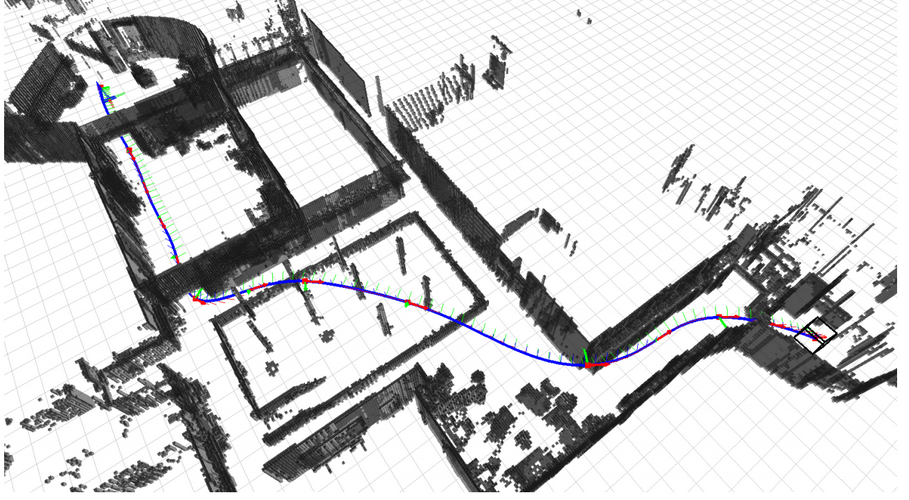
\includegraphics[width=0.6\textwidth]{./images/bry_poly.png}
\caption[Minimum-snap trajectory generation using unconstrained quadratic program]{Minimum-snap trajectory generation using unconstrained quadratic program. \cite{richter2016polynomial}}
\label{fig:bry_poly}
\end{figure}


\subsection{Search-Based Motion Planning}
\label{sec:search_based_planning}
%Search-based Motion Planning for Quadrotors using
%Linear Quadratic Minimum Time Control
Recent work by Kumar et al. \cite{kumar2017search} aims at computing globally optimum, collision-free, minimum-time, dynamically-feasible trajectories in real-time. When the geometric path is first computed and then smoothened, the generated trajectory may not contain a globally optimum trajectory as this approach does not consider the initial dynamics of the robot. As shown in Figure.~\ref{fig:search_kumar}, the trajectory generated by this approach is superior to other approaches. 

\begin{figure}[h!]
\centering
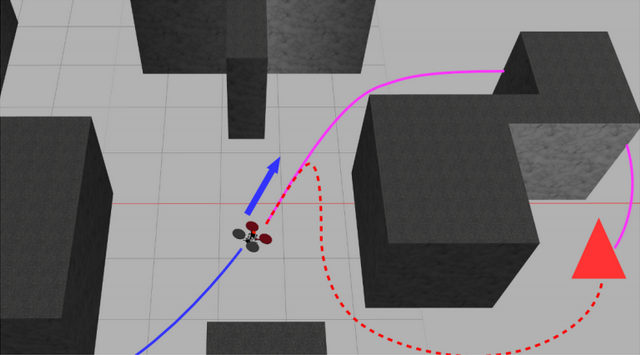
\includegraphics[width=0.6\textwidth]{./images./search_kumar.png}
\caption[Path planning performed at non-zero inital velocity.]{Path planning performed at non-zero initial velocity. The search based approach shown in \cite{kumar2017search} generates the more natural and time optimal magenta curve, where as other approaches gives rise to the red-dashed curve.}
\label{fig:search_kumar}
\end{figure}

Even though others have worked on generating time-optimal trajectories, the algorithms developed were not viable due to their high computational costs. In \cite{kumar2017search}, the algorithm solves an optimal control problem on a set of short-duration motion primitives to explore the space of trajectories. The primitives discretize the state-space into a finite lattice, which is then explored using a graph search algorithm accelerated by a heuristic. Unlike most planning algorithms, this approach doesn't assume an initial hovering condition. Therefore, it is apt for fast replanning when the robot is moving.

% Model Predictive Control
\section{Control of Quadrotors}
\label{sec:control_quadrotors}
Due to the recent popularity of quadrotors, practically all the major control techniques have been used on them. Linear control techniques \cite{seigwart2004pid} have been used to control quadrotors by linearizing their dynamics around an operation point, typically the hover position. The system dynamics is linearized, separating the upward, forward, sideways, and heading, and independent PID controllers control each channel.

Better performance is obtained by non-linear control methods like backstepping, sliding mode \cite{seigwart2005backstepping} and feedback linearization \cite{lewis2009dynamic}. However, an accurate model of the system is necessary for the above-mentioned control techniques to generate satisfactory results. Modelling errors can considerably deteriorate their performance. Adaptive controllers \cite{kumar2011design} perform well in these cases by correcting the errors in model parameter estimates.

\textit{Model predictive control} (MPC) refers to a set of controllers that use a model to compute inputs from the current time to a future time in order to optimise the behaviour of a model along the input trajectory. Since it is a computationally intensive algorithm, it was used in slow systems like chemical plants and oil refineries. Due to the recent increase in computational capabilities, MPC have become popular in robotics. 

MPC is used to generate trajectories interpolating a given set of way-points \cite{singh2001trajectory} by calculating optimal controls online to minimize a cost function within a receding horizon. The constraints of the problem can be incorporated to the optimal control problem (OCP). In \cite{kamel2015fast}, a fast nonlinear model predictive control (NMPC) approach based on a geometric formulation of the error to track the quadrotor's attitude on the SO(3) special orthogonal group. 

Since the constrained optimization problem is computationally intensive, a trade-off has to be made between time horizon and policy lag. This trade-off is alleviated in \cite{neunert2016fast} by solving an unconstrained NMPC problem using Sequential Linear Quadratic (SLQ) solver. By combining trajectory optimization and trajectory contol, this approach generated trajectories of multiple seconds within a few milliseconds. NMPC can seamlessly integrate trajectory tracking, and hence is preferred method for this thesis.

Now that we have introduced the basics of path planning, and its application to single-agent systems, we move ahead to deal with more challenging multi-agent problems in the next chapter. 




